\documentclass[usenatbib,usegraphicx,letterpaper]{mn2e}
\usepackage[totalwidth=480pt,totalheight=680pt]{geometry}

\usepackage{amssymb}
\usepackage{epsfig}
\usepackage{amsmath}
\usepackage{color}

\bibliographystyle{mn2e}

%-------- journals
\newcommand{\araa}{ARAA~}
\newcommand{\apj}{ApJ~}
\newcommand{\apjl}{ApJL~}
\newcommand{\apjs}{ApJS~}
\newcommand{\mnras}{MNRAS~}
\newcommand{\nat}{Nature~}
\newcommand{\physrep}{Phys. Rep.~}
\newcommand{\aj}{AJ~}
\newcommand{\pasp}{ASP~}

%%%% Misc %%%
\newcommand{\beq}{\begin{equation}}
\newcommand{\eeq}{\end{equation}}
\newcommand{\beqray}{\begin{eqnarray}}
\newcommand{\eeqray}{\end{eqnarray}}

\newcommand{\ben}{\begin{enumerate}}
\newcommand{\een}{\end{enumerate}}
\newcommand{\bit}{\begin{itemize}}
\newcommand{\eit}{\end{itemize}}

%%%%%%%%  galaxy properties  %%%%%%%%
\newcommand{\rhalf}{R_{1/2}}
\newcommand{\rhalfdisk}{R_{1/2}^{\rm disk}}
\newcommand{\rhalfbulge}{R_{1/2}^{\rm bulge}}
\newcommand{\adisk}{A_{\rm disk}}
\newcommand{\abulge}{A_{\rm bulge}}
\newcommand{\alphadisk}{\alpha_{\rm disk}}
\newcommand{\alphabulge}{\alpha_{\rm bulge}}
\newcommand{\sigmarhalf}{\sigma_{\rm R_{1/2}}}
\newcommand{\bt}{{\rm B/T}}
\newcommand{\mstar}{M_{\ast}}
\newcommand{\ssfr}{{\rm sSFR}}
\newcommand{\sfr}{{\rm SFR}}

%%%%%%%%  halo properties  %%%%%%%%
\newcommand{\halospin}{\lambda_{\rm halo}}
\newcommand{\mvir}{M_{\rm vir}}
\newcommand{\macc}{M_{\rm acc}}
\newcommand{\mpeak}{M_{\rm peak}}
\newcommand{\zpeak}{z_{\rm peak}}
\newcommand{\mhalo}{M_{\rm halo}}
\newcommand{\rvir}{R_{\rm vir}}
\newcommand{\rmpeak}{R_{\rm M_{peak}}}
\newcommand{\vmaxmpeak}{V_{\rm peak}}

%%%%%%%%  observations  %%%%%%%%
\newcommand{\rproj}{r_{\rm p}}
\newcommand{\wproj}{w_{\rm p}}
\newcommand{\wplarge}{w_{\rm p}^{\rm large}}
\newcommand{\wpsmall}{w_{\rm p}^{\rm small}}
\newcommand{\wpall}{w_{\rm p}^{\rm all}}

%%%%%%%%  units  %%%%%%%%
\newcommand{\kpc}{{\rm kpc}}
\newcommand{\mpc}{{\rm Mpc}}
\newcommand{\msun}{M_\odot}
\newcommand{\kms}{{\rm km/s}}

%%%%%%%%%%%%%%%%%%%%%%%%%%%%%%%%
%%%%%%%%%%%%%%%%%%%%%%%%%%%%%%%%


\usepackage{epsfig}  \usepackage{graphicx}   \usepackage{rotating}

\begin{document}

\title[The Emergent Simplicity of Galaxy Size]
{The Emergent Simplicity of Galaxy Size}


\author[Hearin, Behroozi, Kravtsov \& Moster]{
Andrew Hearin$^{1}$, Peter Behroozi$^{2}$, Andrey Kravtsov$^{3}$, Benjamin Moster$^{4}$\\
$^{1}$Argonne National Laboratory, Argonne, IL, USA 60439, USA\\
$^{2}$Department of Physics, University of Arizona, 1118 E 4th St, Tucson, AZ 85721 USA\\
$^{3}$Department of Astronomy \& Astrophysics, The University of Chicago, Chicago, IL 60637 USA\\
$^{4}$Universit{\"a}ts-Sternwarte, Ludwig-Maximilians-Universit{\"a}t M{\"u}nchen, Scheinerstr. 1, 81679 M{\"u}nchen, Germany
}

\maketitle

\begin{abstract}
We derive empirical modeling constraints on the connection between dark matter halos and the half-light radius of galaxies, $\rhalf.$ Novel to this work, we study galaxy size using new SDSS measurements of the $\rhalf-$dependence of galaxy clustering. We find that smaller galaxies cluster stronger relative to larger galaxies of the same stellar mass, a new result. We show that the $\rhalf-$dependence of galaxy clustering is largely driven by centrals being larger than satellite galaxies of the same halo mass. Stellar mass stripping of satellites has only a mild impact and is unlikely to be the origin of the characteristic magnitude and shape of the clustering signal. Much more successful models are based on the assumption that the mean galaxy profile {\em and its scatter} are correlated with the formation history of the dark matter halo profile. Based on our present findings, we predict that at fixed $\mhalo,$ galaxies with relatively shallow surface brightness profiles reside in relative low-concentration halos, and conversely. In the class of models that give the most faithful recovery of the observed clustering signal, galaxy $\rhalf$ is set by the size of the  virial radius at the time the subhalo reaches its peak halo mass, with log-normal scatter in $\rhalf$ that is strongly correlated with the halo scale radius $R_{\rm s}$ at that time. Our results can be treated as a boundary condition for more complex and fine-grained models of galaxy size, and provide a simple means for cosmological surveys to generate synthetic galaxy populations with realistic sizes across the cosmic web.
\end{abstract}
%Using forward-modeling techniques based on {\tt Halotools}, we confirm previous results in Kravtsov (2013) that $\rhalf$ is well-described by a linear scaling relation with halo virial radius. 

\section{Introduction}
\label{sec:intro}
Some introduction goes here.

\section{Data and Simulations}
\label{sec:data}

Our galaxy sample comes from the catalog of SDSS galaxy profile decompositions provided by \citet{meert_etal15}. This catalog is based on Data Release 10 of the Sloan Digital Sky Survey \citep[SDSS,][]{ahn_etal14}, with improvements to the photometry pipeline and light profile fitting methods \citep{vikram_etal10,bernardi_etal13,bernardi_etal14,meert_etal13}. In the version of this catalog that we use, two-dimensional $r-$band profiles were fit with a two-component de Vaucouleurs + exponential profile to determine the half-light radius $\rhalf.$ We apply the \citet{bell_etal03} mass-to-light ratio to the $r-$band flux and $g-r$ colors in this catalog to obtain an estimate for the total stellar mass $\mstar$ of every galaxy.

We calculate two-point clustering $\wproj$ of our SDSS galaxy sample using line-of-sight projection of $\pi_{\rm max}=20\mpc$ using the {\tt correl} program in {\tt UniverseMachine}. Our results in \S~\ref{sec:results} will give special focus on the dependence of $\wproj$ upon $\rhalf.$ We will quantify this dependence in terms of {\em clustering ratios} of ``large" vs. ``small" galaxies, defined according to whether composite galaxy size is above or below $\langle\rhalf\vert\mstar\rangle,$ computed as the median of a sliding stellar mass window with a width of $N_{\rm gal}=1000.$

As the bedrock of our modeling, we use the catalog of {\tt Rockstar} subhalos identified at $z=0$ in the Bolshoi-Planck simulation \citep{klypin_etal11,behroozi12_rockstar,behroozi12_consistent_trees,riebe_etal13,rodriguez_puebla16_bolplanck}. the particular version of the catalog we use is made publicly available through {\tt Halotools} \citep{hearin_etal16}, with {\tt version\_name} = `halotools\_v0p4'. For mock galaxies, to compute galaxy clustering we employ the distant observer approximation by treating the simulation $z-$axis as the line-of-sight. We compute $\wproj$ using the {\tt mock\_observables.wp} function in {\tt Halotools}, which is a python implementation of the algorithm in the {\tt Corrfunc} C library \citep{sinha_etal17}. 

All numerical values of $\rhalf$ will be quoted in physical $\kpc,$ and all values of $\mstar$ and $\mhalo$ in $\msun,$ assuming $H_0=67.8~\kms\equiv100h~\kms,$ the best-fit value from \citet{planck15}. To scale stellar masses to ``$h=1$ units" \citep{croton13}, our numerically quoted values for $\mstar$ should be multiplied by a factor of $h^2,$ while our halo masses and distances should be multiplied by a factor of $h.$


\section{Galaxy-Halo Model}
\label{sec:model}

\subsection{Stellar mass model}
\label{subsec:model}

We map $\mstar$ onto subhalos with the best-fit stellar-to-halo mass relation from \citet{moster_etal13}:

\begin{equation}
\label{eq:smhm}
\langle\mstar/\mhalo\rangle = 2N\left[(\mhalo/M_{1})^{-\beta} + (\mhalo/M_1)^{\gamma}\right]^{-1}.
\end{equation}
For halo mass $\mhalo$ we use $\mpeak,$ the largest value of $\mvir$ ever attained along the main progenitor branch of the subhalo. 

We additionally explore the potential existence of satellite galaxies that reside in subhalos that are not identified by halo-finder to the present day, so-called ``orphan galaxies" \citep[see, e.g.,][]{campbell_etal17}. We use an extension of {\tt Consistent Trees} that models the evolution of subhalos after disruption. The phase space evolution of orphans is approximated by following a point mass evolving in the host halo potential according to the orbital parameters of the subhalo at the time of disruption; the evolution of subhalo mass and circular velocity is approximated using the semi-analytic model presented in \citet{jiang_vdB14}.   

The values of the best-fit parameters in \citet{moster_etal13} were fit to a stellar mass function (SMF) with values $\mstar^{\rm MPA-JHU}$ based on the MPA-JHU catalog \citep{kauffmann_etal03,brinchmann_etal04}, which differs from the SMF in our galaxy sample \citep[see, e.g.,][]{bernardi_etal14}. We account for this difference by manually tabulating the median value $\langle\mstar^{\rm Meert+15}\vert\mstar^{\rm MPA-JHU}\rangle$ in logarithmic bins spanning $9 < \log_{10}\mstar^{\rm MPA-JHU}/\msun < 12,$ and applying the median correction to the Monte Carlo realization of the mock galaxy sample. This results in a typical boost of $\sim0.25$ dex at $\mstar^{\rm MPA-JHU}\approx10^{9.75}\msun,$ and $\sim0.4$ dex at $\mstar^{\rm MPA-JHU}\approx10^{11.5}\msun.$ 

\subsection{Galaxy size models}
\label{subsec:model}

In \S\ref{sec:results}, we calculate predictions for the $\rhalf-$dependence of galaxy clustering for several different kinds of empirical models, described in turn below.


\subsubsection{K13 model}
\label{subsubsec:k13model}

In \citet{kravtsov13}, it was found that if a stellar-to-halo mass relation is inverted to map halo mass estimates $\mhalo$ onto SDSS galaxies, and then the $\mhalo-\rvir$ relation is applied to map values of $\rvir$ onto the galaxies, then the resulting $\rhalf-\rvir$ relation of SDSS galaxies exhibits the following linear scaling across a wide range of stellar mass:
\beq
\label{eq:fiducial_model}
\rhalf = 0.0125\rvir
\eeq

Motivated by the simplicity of this scaling relation, we transform the \citet{kravtsov13} into a forward model using {\tt Halotools}. For the virial radius of halos and subhalos, we use $\rmpeak,$ the value of $\rvir$ in physical units of $\kpc$ measured at the time of peak subhalo mass, defined by 

\beq
\mpeak\equiv\frac{4\pi}{3}\rmpeak^{3}\Delta_{\rm vir}(\zpeak)\rho_{\rm m}(\zpeak)
\eeq
When generating predictions for the K13 model galaxy sizes, we add uncorrelated log-normal scatter of $\sigmarhalf=0.2$ dex to generate a Monto Carlo realization of the model population. 

\subsubsection{K13 + co-evolution model}
\label{subsubsec:coevolutionmodel}

The {\em K13 + co-evolution model} model is identical to K13, but the scatter in $\rhalf$ at fixed $\rmpeak$ is no longer purely stochastic, but is instead correlated with $\vmaxmpeak.$

 stochastic, while other models will introduce a correlation between the scatter and an additional halo property. Models employing correlated scatter are implemented using the {\tt halotools.empirical\_models.conditional\_abunmatch} function, which generalizes the Conditional Abundance Matching technique described in \citet{hearin_etal13b}. 

\subsubsection{K13 + stripping model}
\label{subsubsec:strippingmodel}

We will also consider models for galaxy size in which stellar mass is stripped from satellite galaxies after infall. The basis of this class of models is the fitting function presented in \citet{smith_etal16}, which was calibrated by studying stellar mass loss in a suite of high-resolution hydrodynamical simulations. In this model, $f_{\ast}$ quantifies the fraction of stellar mass lost as a function of $f_{\rm DM},$ the amount of dark matter that has been stripped since infall:

\beq
f_{\ast} = 1 - \exp(-14.2f_{\rm DM})
\eeq
For $f_{\rm DM}$ we use the ratio of present-day subhalo mass divided by the peak mass, $M_{\rm vir}/M_{\rm peak}.$ If we denote the post-stripping stellar mass as $M_{\ast}',$ then we have $M_{\ast}'\equiv f_{\ast}M_{\ast},$ where $M_{\ast}$ is given by Eq.~\ref{eq:smhm}. We then calculate the post-stripping radius by interpolating $\langle\rhalf'\vert\mstar'\rangle$ directly from SDSS data. 

\section{Results}
\label{sec:results}

In \S\ref{subsec:predictions} we show comparisons between the galaxy size model described in \S\ref{sec:model} and our SDSS sample. We identify the key ingredients that determine the characteristic $\rhalf-$dependence of galaxy clustering in \S\ref{subsec:subsec:shuffle_tests}. In so doing, we demonstrate the sensitivity of galaxy clustering measurements to the underlying model assumptions, establishing the success of our model as non-trivial. 

\subsection{Testing Model Predictions}
\label{subsec:predictions}

In Figure \ref{fig:scatter_plot} we show the scaling of galaxy size $\rhalf$ with $\mstar.$ Scattered gray points show the scaling relation for our SDSS galaxy sample, while the black curve shows the median relation $\langle\rhalf\vert\mstar\rangle$ implied by the model described in \S\ref{sec:model}.

%---------------------------------------------------------------------------------------------------
\begin{figure}
\centering
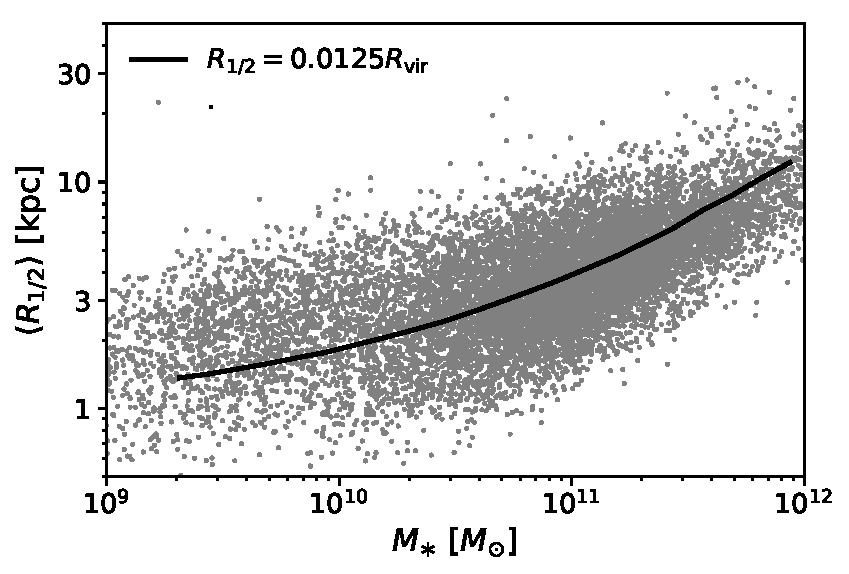
\includegraphics[width=8cm]{FIGS/single_component_model_vs_sdss_one_point.pdf}
\caption{
{\bf One-point data used to fit the fiducial model.}
Scattered points show the $\rhalf-\mstar$ relation for SDSS galaxies as measured in \citet{meert_etal15}. The black curve shows the median $\rhalf-\mstar$ relation implied by the model described in \S\ref{sec:model}, in which $\rhalf=0.0125\rvir.$ This figure confirms the findings in \citet{kravtsov13} that a linear relationship between $\rvir$ and $\rhalf,$ convolved against the nonlinear relationships between $\rvir, \mhalo$ and $\mstar,$ correctly predicts the characteristic curvature in the relation $\langle\rhalf\vert\mstar\rangle$ over a wide range in stellar mass.
}
\label{fig:scatter_plot}
\end{figure}
%-----------------------------------------------------------------------------------------------------

In Figure \ref{fig:clustering_ratio_upshot} we present new measurements of the $\rhalf-$dependence of projected galaxy clustering, $\wproj(\rproj).$ Because galaxy clustering has well-known dependence upon $\mstar$ that is not the subject of this work, we wish to remove this influence and focus purely on the relationship between $\rhalf$ and $\wproj(\rproj).$ To do so, we determine the value $\langle\rhalf\vert\mstar\rangle$ by computing a sliding median of $\rhalf,$ calculated using a window of width $N_{\rm gal}=1000.$ Each galaxy is categorized as either ``large" or ``small" according to whether it is above or below the median value appropriate for its stellar mass. For any $\mstar-$threshold sample, the SMF of the ``large" and ``small" subsamples are identical, by construction. 

We measure $\wproj(\rproj)$ separately for large and small subsamples for four different $\mstar$ thresholds, $\mstar>10^{9.75}\msun,$ $\mstar>10^{10.25}\msun,$ $\mstar>10^{10.75}\msun,$ and $\mstar>10^{11.25}\msun.$ We make the same measurements for each volume-limited $\mstar-$threshold sample {\em without} splitting on size, giving us measurements $\wpall, \wplarge,$ and $\wpsmall$ for each threshold sample. This allow us to compute the ratio $(\wplarge-\wpsmall)/\wpall,$ which we refer to as {\em the $\rhalf$ clustering ratio}. These ratios are the measurements appearing on the y-axis in each panel of Figure \ref{fig:clustering_ratio_upshot}. Points with error bars show SDSS measurements, solid curves show the clustering ratios of model galaxies as predicted by the model described in \S\ref{sec:model}. Before unpacking the information contained in these clustering measurements, we stress that the good agreement shown between model and data in Figure~\ref{fig:clustering_ratio_upshot} is a genuine model prediction, since the model parameters were taken directly from \citet{kravtsov13}, which were fit to the one-point measurements in Fig.~\ref{fig:scatter_plot}, whereas the two-point measurements appearing in Figure \ref{fig:clustering_ratio_upshot} have heretofore never been measured. 

%---------------------------------------------------------------------------------------------------
\begin{figure}
\centering
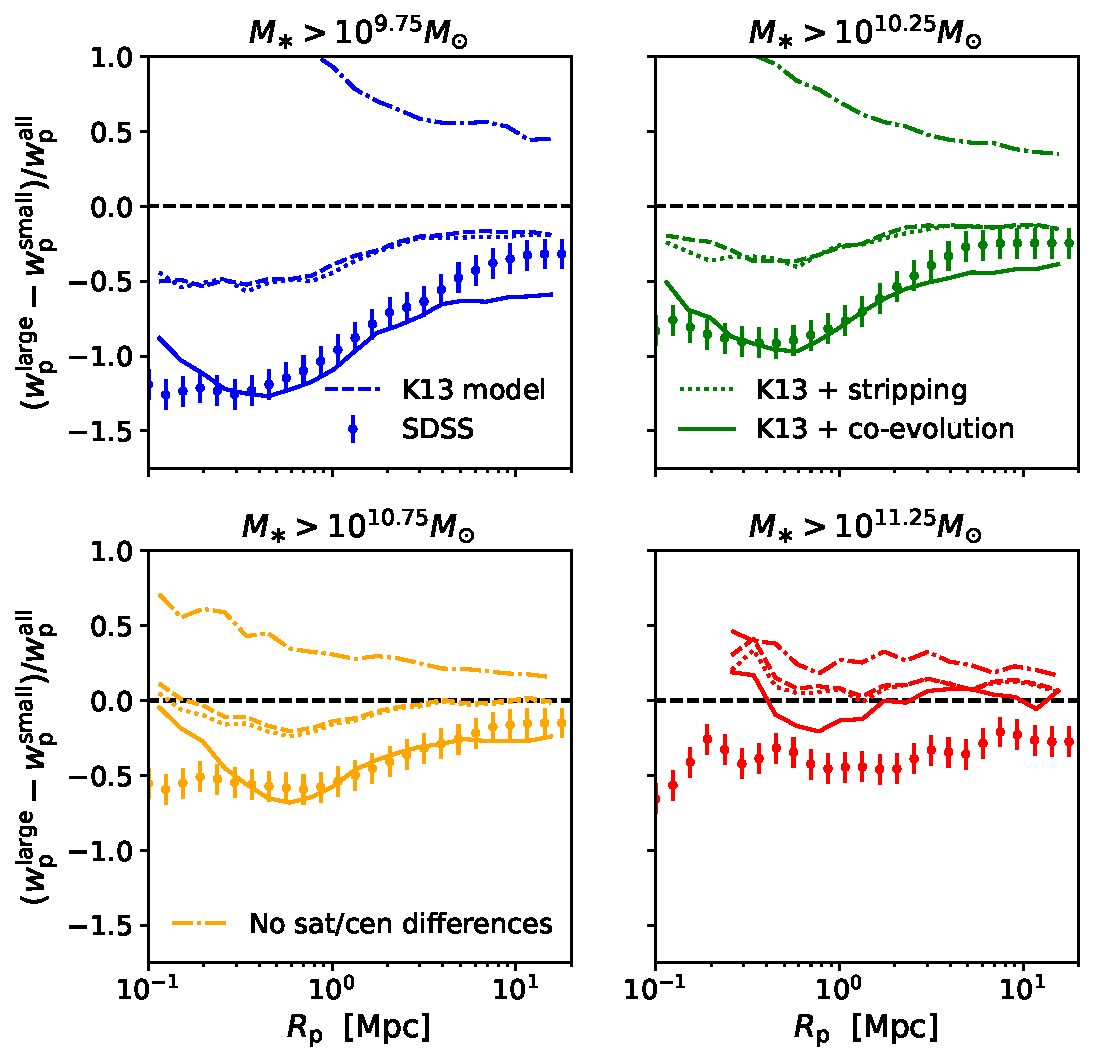
\includegraphics[width=8cm]{FIGS/size_clustering_ratios_stripping_coevolution.pdf}
\caption{
{\bf $\rhalf-$dependence of galaxy clustering.}
Points with error bars show new SDSS measurements of the $\rhalf-$dependence of projected galaxy clustering, $\wproj,$ compared to predictions by the model tuned to the measurements shown in Fig.~\ref{fig:scatter_plot}. We define a galaxy as ``large" or ``small" according to whether it is above or below the median size for its stellar mass, so that in each panel, the SMF of the ``large" and ``small" subsamples are identical, as described in the text. The y-axis shows {\em clustering strength ratios,} so that, for example, a y-axis value of $-0.5$ corresponds to small galaxies being $50\%$ more strongly clustered than large galaxies of comparable stellar mass. Each panel shows results separately for a different volume-limited $\mstar-$threshold samples. See \S\ref{subsec:model} for a description of each model.}
\label{fig:clustering_ratio_upshot}
\end{figure}
%-----------------------------------------------------------------------------------------------------

The salient feature of the clustering ratio measurements is that they are negative: small galaxies cluster more strongly than large galaxies of the same stellar mass, a new result. This feature also holds true for model galaxies. This result may be surprising, since $\rhalf\propto\rvir,$ halo mass $\rvir\propto\mhalo^{1/3},$ and clustering strength increases with $\mvir.$ Based on this simple argument, one would expect the opposite trend to the measurements shown here. We present a resolution to this puzzle in the following section. 

\subsection{Origin of the size-dependence of galaxy clustering}
\label{subsec:shuffle_tests}

%---------------------------------------------------------------------------------------------------
\begin{figure}
\centering
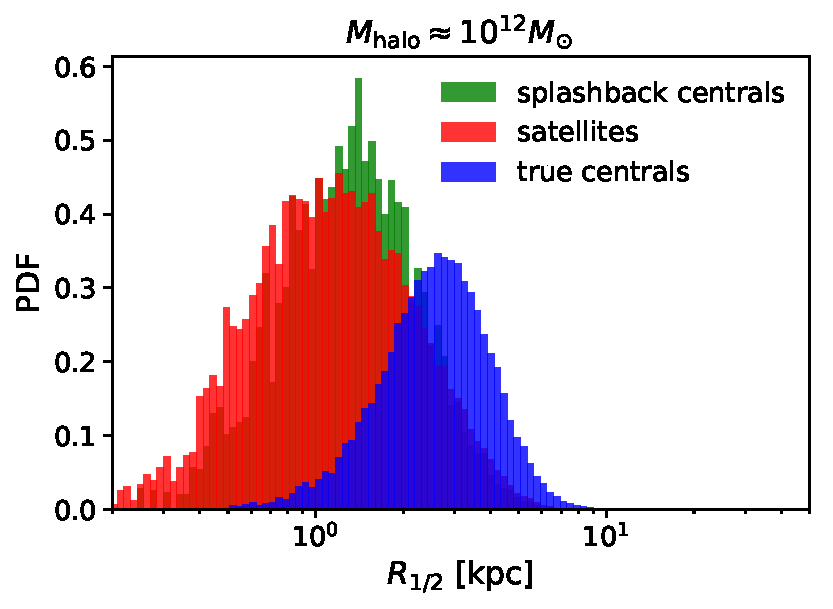
\includegraphics[width=8cm]{FIGS/cen_sat_sizes.pdf}
\caption{
{\bf Relative sizes of centrals and satellites.} In a narrow bin of halo mass $\mhalo=\mpeak\approx10^{12}\msun,$ we show the distribution of model galaxy sizes for different subpopulations galaxies. The red histogram shows the sizes of satellites; the blue histogram shows host halos that have never passed inside the virial radius of a larger halo (``true centrals"); the green histogram host halos that were subhalos inside a larger at some point in their past history (``splashback halos"). In the fiducial model, galaxy size is set by the physical size of the virial radius at the time the (sub)halo attains its peak mass, naturally resulting in smaller sizes for satellites and backsplash centrals relative to true centrals of the same $\mpeak.$
}
\label{fig:shuffle}
\end{figure}
%-----------------------------------------------------------------------------------------------------

%We can understand the origin of the shape of the clustering strength ratios shown in Figure~\ref{fig:clustering_ratio_upshot} through a series of straightforward ``shuffle tests". The points with error bars and solid curves in each panel of Fig.\ref{fig:shuffle} are identical to those appearing in Fig.\ref{fig:clustering_ratio_upshot}, although the dynamic range of the y-axis has changed to accommodate the additional curves. 

%We generated each additional curve by variations on the following exercise. In logarithmic bins of $\mpeak$ with width of $0.1$dex, we randomly shuffle the modeled $\rhalf$ values of some particular subpopulation of model galaxies that reside in subhalos in the $\mpeak$ bin. After repeating this shuffle over the entire range of $\mpeak,$ we then re-divide model galaxies into ``large" and ``small" populations, and remeasure the clustering strength ratios. By shuffling sizes amongst different subpopulations, we can gain an understanding of the subhalo properties that contribute to the characteristic shape of the clustering ratios. 

%In the {\em brown, dotted} curves labeled ``all-gal scramble", we shuffle the sizes of {\em all} model galaxies in the $\mpeak$ bin, so that in the resulting mock, galaxy size has no correlation with any subhalo property beyond $\mpeak.$ In particular, the ``all-gal scramble" mock erases the possible influence of a correlation between galaxy size and the redshift at which the subhalo attains peak mass. The resulting clustering strength ratios become exactly as predicted by the naive expectation sketched at the conclusion of \S\ref{subsec:predictions}: $\rhalf\propto\rvir\propto\mhalo^{1/3},$ and so large galaxies clustering more strongly relative to small galaxies of comparable stellar mass. 

%Statistically, there are actually two distinct effects at work in the ``all-gal scramble".  Central and satellite galaxies of similar $\mpeak$ have their sizes shuffled amongst each other, and the potential influence of central galaxy assembly bias is also erased. We parse these separate effects by exploring three variations on the shuffle tests, described below. 

%For the {\em cyan dashed} curve labeled ``all-cen-scramble", we only shuffle sizes amongst present-day host halos, i.e., amongst subhalos for which Rockstar {\tt upid} equals -1. For the {\em black dashed} curve labeled ``true-cen-scramble", we only shuffle amongst host halos that have never passed within the virial radius of a larger halo throughout their entire assembly history, i.e., we only shuffle amongst non-backsplash host halos. Finally, the {\em purple dot-dashed} curve labeled ``sat-scramble", we only shuffle sizes amongst satellite galaxies, i.e., subhalos that are presently located inside the virial radius of a larger halo. 

% shown in Figure \ref{fig:shuffle}. 


%In light of this explanation, it is natural to ask whether this simple feature {\em alone} is all that is needed for any model of $\rhalf$ to achieve this level of success at predicting galaxy clustering on small and large scales. We address this question in \S~\ref{subsec:tests2} below, finding that the answer is no: the reasonably correct magnitude and scale-dependence of the clustering ratios predicted by our model is a non-trivial result that places tight constraints on the post-infall physics of satellite galaxies.

%We conclude this section by estimating how satellite mass stripping manifests in $\wproj(\rproj).$ To do so, we construct an extension our fiducial model with a simple additional ingredient for post-infall evolution of satellites mass and size. 

%In the fiducial model described in \S~\ref{sec:model}, recall that in the power law a scaling relations (Eq.~\ref{eq:fiducial_model}) the halo radius $\rvir$ used for satellite galaxies is taken to be the value at the time of infall. The simple interpretation of this assumption is that, in a statistical sense, the size of satellite galaxies is determined by its history as a central galaxy, and that post-infall physics leaves no distinct imprint on satellite $\rhalf.$

%Here we suppose that this assumption is violated, and that $\rhalf$ decreases after infall according to $(\mvir/\macc)^{1/3}.$ That is, in this alternative formulation, rather than using $\rvir$ at the time of infall for satellites in the power law scaling relations, we instead use $\rvir(\mvir/\macc)^{1/3}.$ This simple toy model attempts supposes that the same physical processes leading to halo mass loss are also responsible for a post-infall decrease in satellite size.

%---------------------------------------------------------------------------------------------------
\begin{figure}
\centering
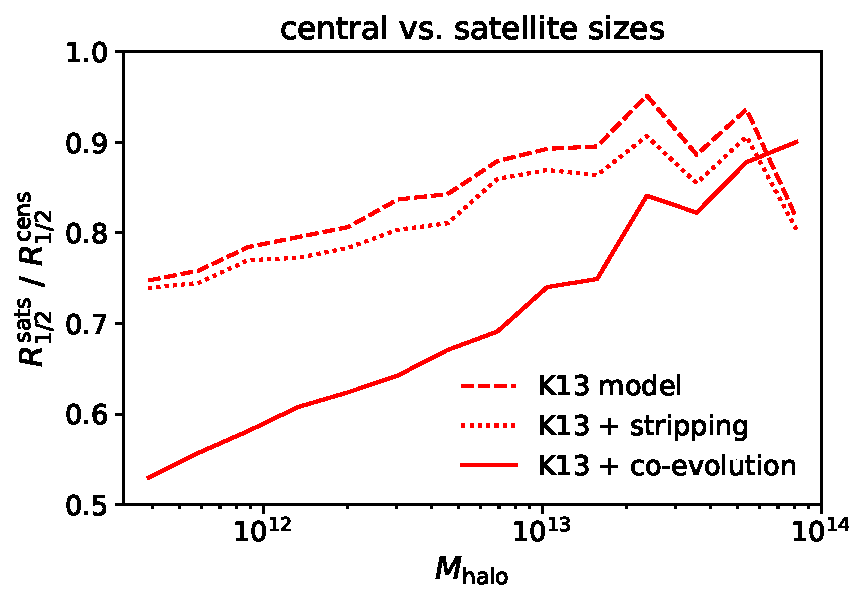
\includegraphics[width=8cm]{FIGS/sat_vs_cen_sizes_fracdiff.pdf}
\caption{
{\bf Origin of the $\rhalf-$dependence of clustering.}
Here we compare our fiducial model, in which satellite galaxy size is set by $\rvir$ at the time of infall, to a set of alternative models created by shuffling the sizes of various subsamples of the fiducial mock. 
}
\label{fig:shuffle}
\end{figure}
%-----------------------------------------------------------------------------------------------------

%Figure~\ref{fig:satellites} compares the clustering ratios of our fiducial model (solid curves) to the clustering ratios of this alternative model (dashed curves). The difference between the small-scale clustering of the two models is stark: the assumption that $\rhalf$ decreases after infall leaves a strong imprint on the $\rhalf-$dependence of $\wproj(\rproj),$ such that small galaxies cluster {\em much} more strongly relative to large galaxies, particularly for disk-dominated systems with $\mstar\approx10^{10}\msun.$

%The large differences between the solid and dashed curves in Fig.~\ref{fig:satellites} establishes that the largely successful prediction for the clustering ratios fiducial model is a non-trivial: $\wproj(\rproj)$ is indeed providing good constraining power on the  assumptions underlying our profile modeling and not simply our morphology modeling, c.f., \S\ref{subsubsec:random_bt_model} and \S\ref{sec:model}. We refer the reader to \S\ref{subsec:satellite_discussion} for further discussion of the physical implications of this result.

\section{Discussion}
\label{sec:discussion}

\subsection{Progression from Backwards to Forwards Modeling}
\label{subsec:forwardsmodeling}

\subsection{Implications for Satellite Mass Loss}
\label{subsec:satellite_discussion}

\subsection{Future Directions for Empirical Modeling of Morphology}
\label{subsec:future}


\section{Conclusions}
\label{sec:conclusion}

\subsection{Summary}
\label{subsec:summary}

\section*{Acknowledgments}

APH thanks John Baker for the {\em Toejam \& Earl} soundtrack. 

\bibliography{galsize_paper}

\end{document}







